\section{Обзор предметной области}

Одним из основных подходов к заданию принтеров являются принтер-комбинаторы.
В этой главе приведен обзор классических принтер-комбинаторов, а также
принтер-комбинаторов с дополнительным оператором \emph{выбора}, которые
в рамках данной работы использованы для реализации принтеров, задаваемых
с помощью шаблонов. Для решения проблем эффективности
комбинаторов с выбором в данной работе был использован подход BURS.
Апробация подхода задания принтеров с помощью шаблонов
была произведена для языка Java, для которого есть средства форматирования,
встроенные в IDE.

\subsection{Принтер-комбинаторы}

Базовыми принтер-комбинаторными библиотеками являются библиотеки
Джона Хьюза\cite{hughes} и Филиппа Вадлера\cite{wadler}, которые
представляют собой функциональную переработку алгоритма
Оппена\cite{oppen}.
Ограничимся рассмотрением библиотеки Вадлера, так как
библиотека Хьюза обладает теми же свойствами, которые принципиальны в контексте
данной работы.

В библиотеке ключевым типом является документ.
Он представляет сущность, которая потом может
быть переведена в строковое представление алгоритмом принтера.
Основные конструкторы для составления документа таковы:
\begin{itemize}
  \item атомарная строка, которая печатается как есть;
  \item \emph{разделитель};
  \item последовательная композиция двух документов;
  \item набор связанных документов.
\end{itemize}

Определяющей особенностью данного подхода является то, что все разделители
в рамках одного набора могут быть совместно заменены алгоритмом принтера
на пробельный символ или на перевод строки. Выбор для каждого набора разделителей
основывается на том, что вывод должен поместиться в заданную ширину,
используя минимальное число строк.

Основная проблема такого подхода заключается в его слабой выразительной силе.
Документы, построенные по синтаксическому дереву печатаемой программы,
обрабатываются слишком единообразно, что иногда приводит к нежелательному результату.
Пусть, к примеру, нужно напечатать программу на языке
Python\footnote{\cd{http://python.org}}.
Между последовательными операторами в случае их печати на одной строчке необходимо
добавить дополнительный разделитель (``;''), иначе программа станет некорректной
(см. рис.~\ref{fig:seqEx}). Однако, описанные принтер-комбинаторы не предоставляют
возможности задать такое поведение.
Кроме того, с помощью таких принтер-комбинаторов невозможно выразить разные проектные СК,
так как они всегда печатают текст в одном стиле, который жестко ``зашит'' в их код.

\begin{figure}[h!]
	\centering
	\null\hfill
	\subfloat[Корректный код]{
		\centering
    \makebox[.4\textwidth] {
		  \lstinputlisting[language=Python]{codes/pythonCode.py}
    }
	}
	\null\hfill
	\subfloat[Некорректный код]{
		\centering
    \makebox[.4\textwidth] {
	  	\lstinputlisting[language=Python]{codes/pythonCodeBad.py}
    }
	}
	\hfill\null
	\caption{Пример работы принтер-комбинаторов для языка Python}
  \label{fig:seqEx}	
\end{figure}

Более подробный обзор библиотек Хьюза и Вадлера представлен в \cite{myCoursePaper}.

Большинство принтер-комбинаторных библиотек\cite{
swierstraChitil, swierstra04, peytonJones, kiselyov, chitil}
являются развитиями работ Хьюза и Вадлера. Так, в отличие от базовых, среди
них есть реализации с линейной сложностью обработки документа от его размера и
\emph{online} алгоритмы, которые не требуют просмотра всего документа
для начала печати его текстового представления. Но все они обладают тем же
интерфейсом, а значит в них также неразрешимы задачи, в которых требуется
задавать варианты текстовых представлений, которые отличаются не только
пробелами и переводами строк.

\subsection{Принтер-комбинаторы с выбором}

Существенно от описанных выше отличаются библиотеки, предоставляющие в своем
интерфейсе комбинатор \emph{выбора}, который позволяет задавать для одного поддерева
принципиально разные варианты раскладок.
Так, в работах~\cite{jongeEveryOccasion, jongeReengine} используется оператор ``ALT'',
но алгоритм принтера устроен так, что среди двух альтернатив выбирается первая, если она
помещается в заданную ширину, и вторая --- иначе,
что не дает оптимальный результат на выходе.

Оптимальные принтер-комбинаторы с выбором были впервые представлены в работе~\cite{swierstra}.
Их реализация является частью Utrecht Tools
Library\footnote{\cd{http://www.cs.uu.nl/wiki/HUT/WebHome}}
(практическая реализация несколько изменена по
отношению к той, что описана в статье, но отличие несущественно).
В данном подходе текст строится из блоков прямоугольной формы с возможно неполной последней
строчкой (см. рис. \ref{fig:basicFormat}). В реализации на Haskell блоки представляются
структурой \lstinline[language = Haskell]{Format}:
\begin{lstlisting}
    data Format = Elem { height        :: Int
                       , lastLineWidth :: Int
                       , width         :: Int
                       , txtstr        :: Int -> String -> String
                       }
\end{lstlisting}

Первые три поля структуры определяют геометрические размеры блока, а последнее --- функция,
которая используется для преобразования блока в текст. Здесь используется функция, а не
просто строчка, чтобы можно было преобразовывать вложенные блоки за линейное время. Первый
аргумент \lstinline[language = Haskell]{txtstr} задает сдвиг блока.

\begin{figure}
  \centering
  \subfloat[Блок текста]{
    \raisebox{5mm}{
      \centering
      \vspace{0pt}
      \tikz[scale = 2.0]{
        \draw (0,0) -- (1,0) -- (1,0.2) -- (2,0.2) -- (2,1) -- (0, 1) -- cycle;
      }
    }
    \label{fig:basicFormat}
  }
  ~
  \subfloat[Горизонтальная композиция]{
    \centering
    \tikz[scale = 2.0]{
       \draw (0,0) -- (1,0) -- (1,0.2) -- (2,0.2) -- (2,1) -- (0, 1) -- cycle;
       \draw (1.1,-0.9) -- (2.1,-0.9) -- (2.1,-0.7) -- (3.1,-0.7) -- (3.1,0.1) -- (1.1,0.1) -- cycle;
     }
     \label{fig:beside}
  }
  %\hfill
  ~
  \subfloat[Вертикальная композиция]{
    \makebox[.28\textwidth] {
    \centering
    \tikz[scale = 2.0]{
       \draw (0,0) -- (1,0) -- (1,0.2) -- (2,0.2) -- (2,1) -- (0, 1) -- cycle;
       \draw (0,-1.1) -- (1,-1.1) -- (1,-0.9) -- (2,-0.9) -- (2,-0.1) -- (0,-0.1) -- cycle;
    }
    \label{fig:above}
    }
  }
  \caption{Примитивы структуры Format}
  \label{fig:basicConcat}
\end{figure}

Для работы с блоками текста используется следующие четыре примитива:
\begin{lstlisting}
    s2fmt     :: String -> Format
    indentFmt :: Int -> Format -> Format
    aboveFmt  :: Format -> Format -> Format
    besideFmt :: Format -> Format -> Format
\end{lstlisting}

Функция \lstinline[language = Haskell]{s2fmt} создает блок текста,
состоящий из одной строчки; \lstinline[language = Haskell]{indentFmt} по блоку создает новый,
сдвинутый на заданное число позиций. Действие примитивов композиции
\lstinline[language = Haskell]{besideFmt} и \lstinline[language = Haskell]{aboveFmt}
показано на рис.~\ref{fig:beside} и \ref{fig:above} соответственно.

Также, как и в библиотеках без комбинатора выбора, в работе~\cite{swierstra} используется понятие
\emph{документа}. Здесь документ можно рассматривать как множество возможных раскладок
(набор \lstinline[language = Haskell]{Format}-элементов). Документы описываются типом
\lstinline[language = Haskell]{Doc}, который на этапе построения представляет собой
дерево применений комбинаторов (приведены ниже), а на этапе обработки алгоритмом
принтера ему в соответствие ставится итоговое множество вариантов.

Документ конструируется с помощью следующих комбинаторов, которые симметричны
примитивам построения блоков текста:
\begin{lstlisting}
    text   :: String -> Doc
    indent :: Int -> Doc -> Doc
    beside :: Doc -> Doc -> Doc
    above  :: Doc -> Doc -> Doc
\end{lstlisting}

В дополнение появляется пятый комбинатор для документов:
\begin{lstlisting}
    choice :: Doc -> Doc -> Doc
\end{lstlisting}

Этот комбинатор и является тем самым комбинатором выбора. Он представляет
\emph{объединение} множеств раскладок документов, которые были переданы как
аргументы комбинатора. Заметим, что только этот комбинатор может произвести
документ с несколькими раскладками из одновариантных аргументов.

Оригинальная реализация существенно опирается на ленивые вычисления. В \cite{swierstra}
множество вариантов, соответствующее экземпляру \lstinline[language = Haskell]{Doc},
представляется ленивым списком всех возможных раскладок, удовлетворяющих ограничению
на максимальную ширину. Этот список отсортирован в порядке ``ухудшения''
раскладок, то есть в голове списка лежит ``лучшая'', в терминах оптимальности,
раскладка из возможных при заданной ширине. В случае
\lstinline{beside}- и
\lstinline{above}-композиций
документов полная (без учета ленивости) сложность вычисления списка нового документа
составляет $O(n \times m)$, где $n$ и $m$ --- размеры списков, соответствующих 
соединяемым документам; размер нового списка также $n \times m$.

Выбор лучшего представления для самого верхнеуровнего документа происходит
просто --- нужно из соответствующего списка взять первый элемент. Поэтому
на первый взгляд кажется, что общее число операций,
благодаря ленивым вычислениям, существенно уменьшается.
Но это не так из-за реализации обработки документа,
построенного с помощью комбинатора \lstinline[language = Haskell]{beside}, которая
форсирует полное вычисление дочерних списков. Более того, из-за свойств отношения
порядка, построенного по критерию оптимальности, в рамках данной модели списков
принципиально нельзя построить ленивую обработку комбинатора
\lstinline[language = Haskell]{beside}.
Так, выбор оптимальной раскладки документа в
\cite{swierstra} имеет в худшем случае экспоненциальную сложность от числа
комбинаторов, использованных при его построении.
В \cite{swiComb} приведены оптимизации для данной модели, но они
не улучшают асимптотику решения для деревьев в общем случае.

\subsection{BURS}

Bottom-Up Rewrite System (BURS)\cite{burs} --- это метод динамического
программирования на деревьях, изначально появившийся в контексте задачи выбора
набора инструкций для генерации машинного кода. Основой BURS является
регулярная древесная грамматика\cite{tata} со стоимостью применения подстановки,
то есть грамматика со следующим набором правил: 

$$
\begin{array}{rcll}
  N &:& \alpha& [c]\\
  N &:& \alpha\; (K_1,\dots,K_n)& [c]
\end{array}
$$

Здесь $N, K_i$ это нетерминалы, $\alpha$ --- терминал,
$c$ --- функция цены, описанная для каждого правила.
Как и для обычной линейной грамматики, вводится стартовый
нетерминал S. Считается, что терминальное дерево выводится в
данной грамматике, если его можно получить с помощью правил
подстановки из одноузлового дерева $S$.
Каждая подстановка заменяет нетерминал $N$, находящийся в листе дерева, на дерево 
$\alpha\;(K_1,\dots,K_n)$, если в грамматике есть правило
$N:\alpha\;(K_1,\dots,K_n)$. 
Для каждой подстановки вычисляется стоимость ее применения с помощью
функции цены ($c$).
Аргументами функции могут служить терминальная метка ($\alpha$) и стоимости
вывода поддеревьев.
Задачей, которую решает BURS, является поиск вывода наименьшей стоимости
для заданного дерева по заданной грамматике.
Такой вывод может быть найден двухпроходным алгоритмом.

Первый проход (\emph{пометка}) обрабатывает дерево снизу вверх и вычисляет
для каждого узла набор троек $(K,\;R,\;c)$, где $K$ --- нетерминал, из которого может быть
выведено поддерево с корнем в обрабатываемом узле,
$R$ --- первое правило, которое используется для вывода минимальной стоимости из $K$,
$c$ --- стоимость такого вывода.
Процесс пометки происходит следующим образом:

\begin{itemize}
\item для листовой вершины, помеченной терминалом $\alpha$, в множество троек
этого вершины добавляется $(K,\;R,\;c\:(\alpha))$ для каждого правила $R=K:\;\alpha\;[c]$;
\item для промежуточной вершины, помеченной терминалом $\alpha$,
с непосредственными поддеревьями $v_1,\dots,v_n$
в множество добавляется тройка $(K,\;R,\;c\:(\alpha,c_1,\dots,c_n))$ для каждого правила
$R=K:\;\alpha\;(K_1,\dots,K_n)\;[c]$, где $(K_i,\;R_i,\;c_i)$ входит в множество троек для
$v_i$; если есть несколько правил вывода из нетерминала $K$, то выбирается правило,
минимизирующее стоимость вывода.
\end{itemize}

Второй проход (\emph{свертка}) просматривает дерево сверху вниз, используя сделанные пометки.
Первое правило из минимального вывода определяется тройкой $(S,\;R,\;c)$ для корневого узла
(если такой тройки нет, то вывод из $S$ невозможен).
Это правило однозначно определяет нетерминалы $K_i$ для каждого непосредственного поддерева
и процесс повторяется.

Для пометки дерева потенциально необходимо каждое правило грамматики применить к каждому узлу.
При фиксированной грамматике алгоритмическая сложность первого прохода --- $O\:(|R|)$,
где $|R|$ --- количество правил
(размер множества троек для каждого узла ограничен числом нетерминалов, которое не больше,
чем количество правил). Свертка также имеет линейную сложность.


\newpage
\subsection{Средства форматирования кода в IDE}

Интегрированные среды разработки программного обеспечения
(IDE) предоставляют средства
для форматирования программного кода. Рассмотрим их на примере двух Java IDE ---
IntelliJ IDEA и Eclipse\footnote{\cd{http://eclipse.org}}.
Для задания требуемого СК используется широкий набор настроек \emph{форматтера},
подпрограммы IDE, отвечающей за форматирование исходных текстов.
Примерами таких настроек являются:
\begin{itemize}
  \item помещать ли фигурную скобку на той же строке, что и
    предыдущее выражение;
  \item форматирование списков --- всегда на одной строчке, переводить строчку после
    каждого элемента или печатать на одной строке,
    пока строчка меньше заданной рекомендуемой ширины;
%   \item и т.д.
\end{itemize}
На рис. ~\ref{fig:ideaFormatter} и~\ref{fig:eclipseFormatter} приведены диалоги задания
параметров форматирования в IntelliJ IDEA и Eclipse соответственно.

\begin{figure}[p]
	\centering
	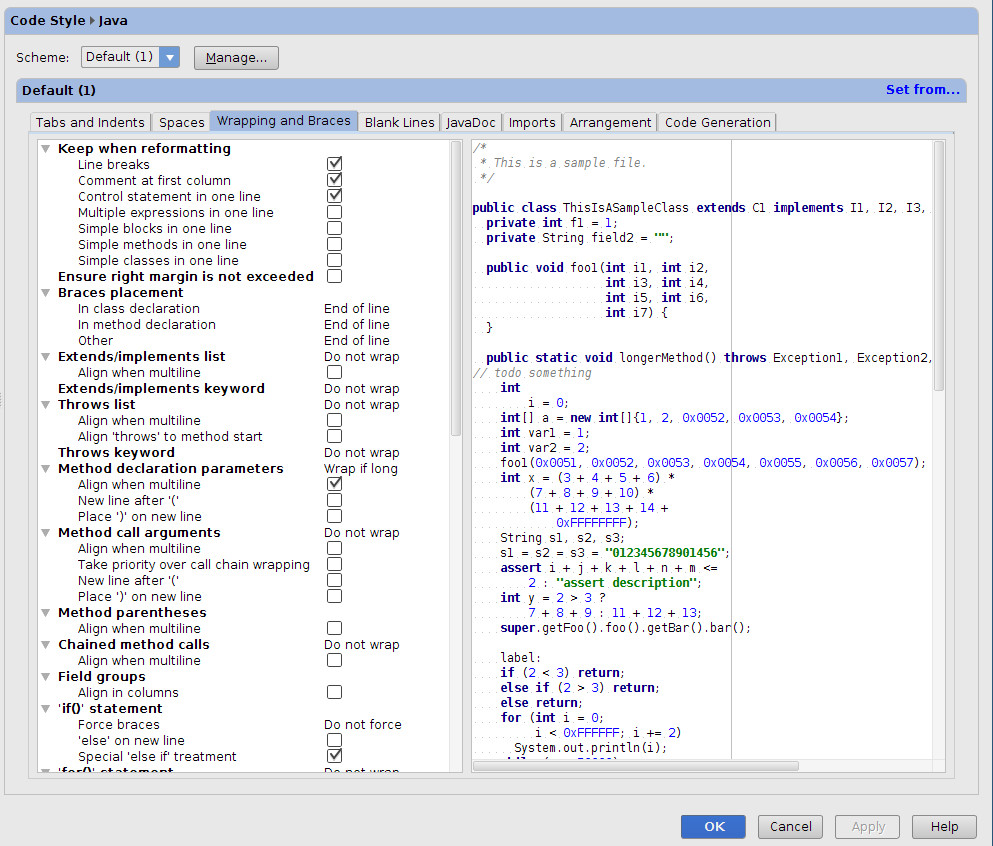
\includegraphics[width=\textwidth]{ideaFormatter}
	\caption{Окно настройки форматтера IntelliJ IDEA}
	\label{fig:ideaFormatter}
\end{figure}

\begin{figure}[p]
	\centering
	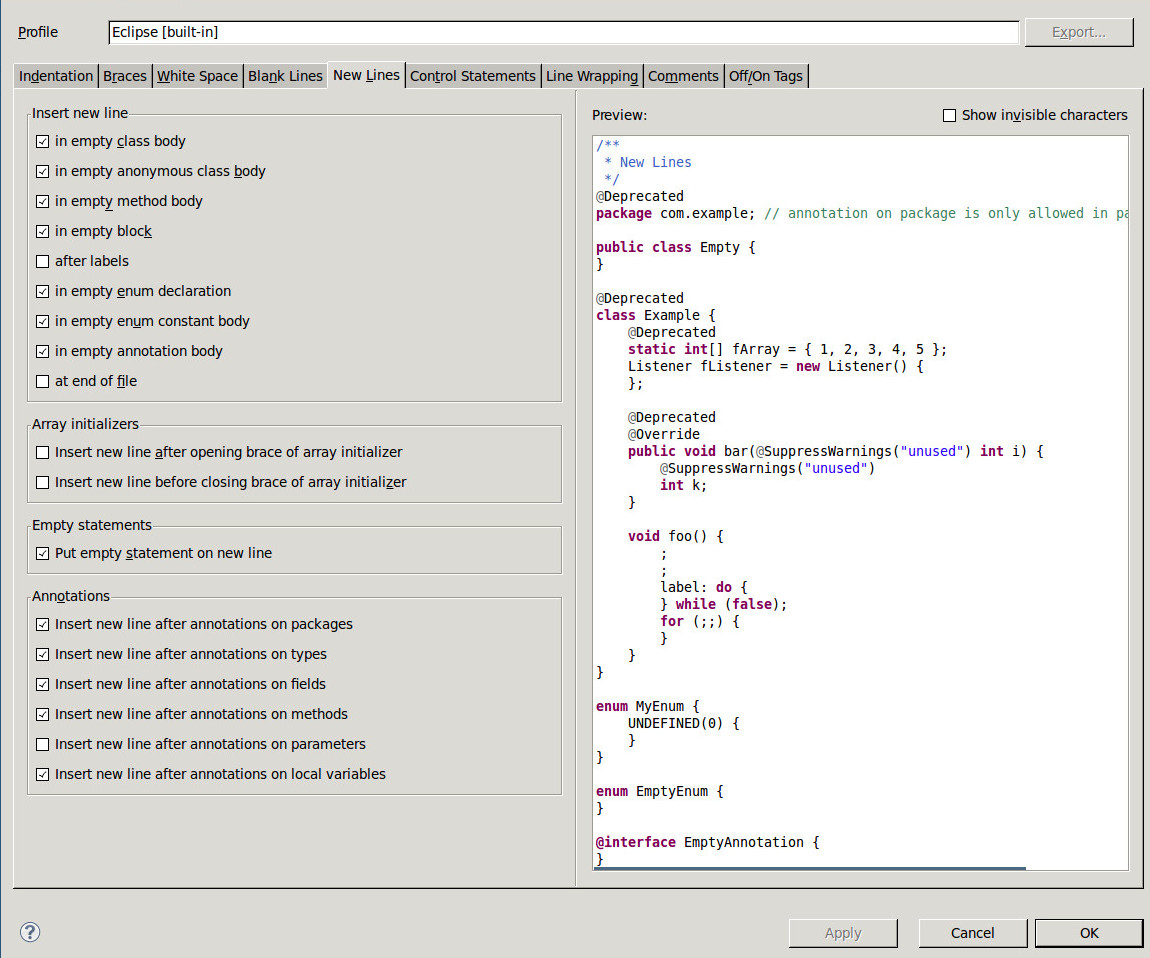
\includegraphics[width=\textwidth]{eclipseFormatter}
	\caption{Окно настройки форматтера Eclipse}
	\label{fig:eclipseFormatter}
\end{figure}

У встроенных форматтеров есть следующие особенности.
Во-первых, это невозможность выразить
оригинальный СК, так как настройки форматтеров, несмотря на их большое
количество,
дают ограниченную вариативность для текстовых представлений форматируемых
программ. В целом, количество принципиально разных
стилей форматирования, которые можно задать с помощью данных настроек,
невелико.
Во-вторых, в случае если надо
придерживаться СК уже существующего проекта, то по коду этого проекта необходимо
вручную задать все настройки форматтера.
Причем наборы настроек в разных IDE не совпадают, что увеличивает сложность
поддержки единого СК, если разработчики используют отличные от друг друга IDE.
Для решения данной проблемы существуют плагины, позволяющие использовать
внешние фоматтеры\footnote{\cd{http://plugins.jetbrains.com/plugin/6546}}.
Кроме того, есть средства, позволяющие экспортировать настройки форматтера в
XML-файл, для их использования в другой
IDE\footnote{\cd{http://blog.jetbrains.com/idea/2014/01/intellij-idea-13-importing-code-formatter-settings-from-eclipse/}}.

Важным достоинством описанных принтеров является малое время работы.
Это достигается в том числе и за счет того, что часто форматируется не весь
файл, а только его часть (см. \cite{eclipse}),
и из-за детерминированности представлений узлов синтаксического дерева,
которая следует из специфики настроек форматтера.
Однако форматирование целого большого проекта занимает существенное время.
Например, обработка кода IntelliJ IDEA Community Edition занимает более часа
у встроенного в IDEA форматтера.

